\section{Introduction}

Today's client-server based file system metadata services have scalability
problems. It takes a lot of resources to server POSIX metadata requests and
applications perform better with dedicated metadata
servers~\cite{sevilla:sc15-mantle, ren:sc2014-indexfs}. This is fine for small
workloads and file systems but as the system scales provisioning a metadata
server for every client is expensive and complicated.

Current hardware evolution and the rise of software-defined storage storage,
which uses techniqes like erasure coding, replication, and partitioning, have
ushered a new era of HPC computing; architectures are transitioning from
complex storage stacks with burst buffer, file system, object store, and tape
tiers to a two layer stack with just a burst buffer and object
store~\cite{bent:login16-hpc-trends}. This trend exacerbates the metadata
scalability problem and has given rise to the serverless metadata services.
%\begin{listing}
\begin{minted}{python}
def hello():
\end{minted}
%\caption{JSON example} 
%\label{json-example}
%\end{listing}

HPC workloads are so metadata intensive that new management techniques are
advocating reducing synchronization and serialization overheads by transferring
these responsibilities to the client. We call this approach decoupling the
namespace and the semantics of consistency differ amongst systems.

\begin{figure}[tb]
\centering
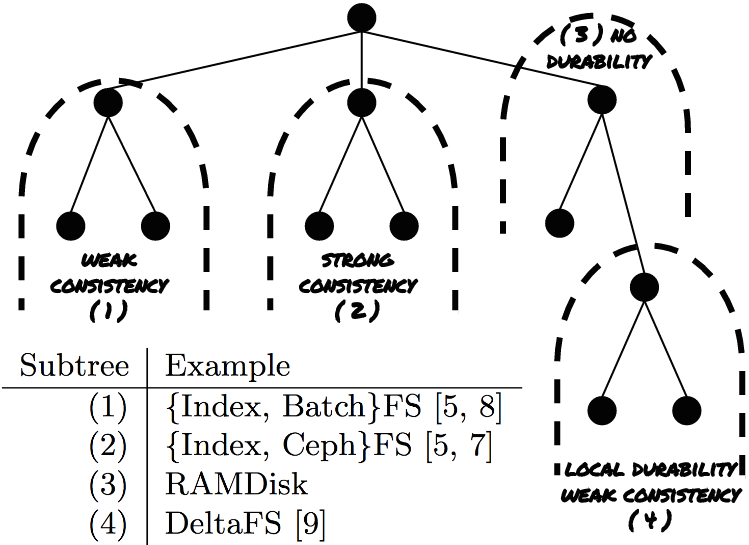
\includegraphics[width=75mm]{figures/subtree-policies.png}
\caption{Administrators can assign consistency and fault tolerance policies to
subtrees to get the benefits of some of the state-of-the-art HPC architectures.
}\label{fig:subtree-policies}
\end{figure}

We propose subtree policies, an interface that lets future programmers control
how the system manages different parts of the namespace.  For performance one
subtree can adopt weaker consistency semantics while another subtree can retain
the rigidity of POSIX's strong consistency. Figure~\ref{fig:subtree-policies}
shows an example setup where a single global namespace has directories for
applications designed for different, state-of-the-art HPC architectures.  Our
system supports 3 forms of consistency and 2 forms of fault tolerance giving
the administrator a wide range of policies and optimizations depending on the
application's needs.


